%% hf: enable header and footer.
\documentclass[
% hf, % <-- Not sure if this should be enabled
]{ceurart}

% One can fix some overfills
% \sloppy

% This was used to mitigate some warnings
\usepackage[T1]{fontenc}
\usepackage{lmodern}

\begin{document}

% Rights management information. CC-BY is the default license.
\copyrightyear{2024}
\copyrightclause{Copyright for this paper by its authors.
  Use permitted under Creative Commons License Attribution 4.0
  International (CC BY 4.0).}

\conference{BPM 2024: Demos and Resources, September 01-06, 2024, Krakow, PL}

\title{BPMN Analyzer 2.0: Instantaneous, Comprehensible, and Fixable Anomaly Detection for BPMN Models}

\author[1]{Tim Kräuter}
[email=tkra@hvl.no]
\author[1]{Patrick Stünkel}
[email=past@hvl.no] % patrick.stuenkel@hvl.no
\author[1]{Adrian Rutle}
[email=aru@hvl.no]
\author[1]{Yngve Lamo}
[email=yla@hvl.no]
\author[2,1]{Harald König}
[email=harald.koenig@fhdw.de]
\address[1]{Western Norway University of Applied Sciences, Bergen, Norway}
\address[2]{FHDW Hannover, Germany}

\begin{abstract}
% 102 words
Many business process models have control-flow anomalies, such as deadlocks or livelocks, which hinder proper execution.
In this paper, we introduce a new tool that can instantaneously identify anomalies in BPMN models, make them understandable for modelers, and suggest corrections to resolve them.
We demonstrate that detection is instantaneous by benchmarking our tool against synthetic BPMN models with increasing size and state space complexity, as well as realistic models.
Moreover, the tool directly displays detected anomalies in the model, including an interactive visualization, and suggests fixes to resolve them.
The tool is open-source, extensible, and integrated into a popular BPMN modeling tool.
\end{abstract}

\begin{keywords}
BPM,
Verification,
Control-flow Analysis,
BPMN model checking,
Soundness,
Safeness
\end{keywords}

% TODO: Soundness vs anomaly detection? Maybe use soundness and say later that in the UI, it's not called soundness!

\maketitle
% 5 pages including references

\section{Introduction}

% Problem statement
Business Process Modeling Notation (BPMN) is becoming increasingly popular for automating processes and orchestrating people and systems.
However, many process models suffer from control-flow anomalies, such as deadlocks, livelocks, starvation, and lack of synchronization~\cite{fahlandAnalysisDemandInstantaneous2011}.
These errors hinder the correct execution of BPMN models and may be detected late in the development process, resulting in elevated costs.

% Solution
In this paper, we describe a new tool, the \textit{BPMN Analyzer 2.0}\footnote{
In the following, we will use BPMN Analyzer to refer to the BPMN Analyzer 2.0, not our previous BPMN Analyzer described in \cite{krauterFormalizationAnalysisBPMN2023}.}, for analyzing BPMN process models to detect control-flow anomalies \textit{already} during modeling.
\autoref{fig:overview} shows an overview of the tool.
The tool front-end is based on the popular \textit{bpmn.io} ecosystem, while the analysis is implemented in Rust for performance and memory efficiency reasons.
The BPMN Analyzer is open-source and accessible online\footnote{\url{https://timkraeuter.com/bpmn-analyzer-js/}} alongside a video demonstration\footnote{\url{https://www.youtube.com/watch?v=MxXbNUl6IjE}}~\cite{timkrauterBPM2024Artifacts2024}.

\begin{figure}[ht]
	\centering
	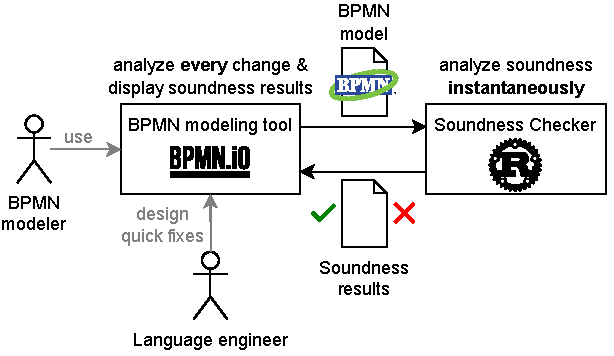
\includegraphics[width=0.6\linewidth]{images/overview}
	\caption{Overview of the BPMN Analyzer 2.0}
	\label{fig:overview}
\end{figure}

The tool can check models after each change since analysis is \textit{instantaneous} according to \cite{fahlandAnalysisDemandInstantaneous2011}, i.e., it takes 500ms or less.
Furthermore, we ensure the results are \textit{comprehensible} by highlighting possible violations directly in the model and displaying an interactive counterexample visualization.
Finally, the tool suggests \textit{fixes} for the most common soundness violations and can be extended to suggest more fixes in the future.
However, the BPMN analyzer cannot provide fixes for all possible violations due to the wide variety of possible control-flow anomalies in BPMN models.

% Why is it significant for the BPM field?
Fahland et al.~\cite{fahlandAnalysisDemandInstantaneous2011} describe \textit{coverage}, \textit{immediacy}, and \textit{consumability} as the main challenges for users unaccustomed to formal analysis methods.
The BPMN Analyzer addresses all these challenges since it supports the most common BPMN elements used in practice (coverage), provides \textit{instantaneous} results (immediacy), and a \textit{comprehensible} user interface (consumability), even including suggestions of fixes.
Developers of industrial BPMN solutions also like our tool, especially the End-2-End user journey\footnote{\url{https://forum.bpmn.io/t/automatic-bpmn-control-flow-analysis-and-resolution/11150}}.
Thus validating our claim of a UI that is understandable for users unfamiliar with formal analysis methods.

% Paper structure
In the remainder of the paper, we describe how instantaneous, comprehensible, and fixable anomaly detection is achieved in \autoref{sec:innovations}.
Then, we discuss the maturity of our tool in \autoref{sec:maturity} before presenting related work in \autoref{sec:related-work}.
Finally, we conclude in \autoref{sec:conclusion}.

% Must have section according to the description
% A section discussing the innovations of the tool or resource to the BPM community and its main characteristics or features
\section{Innovations} \label{sec:innovations} % Main tool description and showing the innovations
The BPMN Analyzer has three main innovations: \textbf{instantaneous}, \textbf{comprehensible}, and \textbf{fixable} anomaly detection.
In this section, we will present the innovations, and more details can be found in our extended paper \cite{krauterInstantaneousComprehensibleFixable2024}.
% Instantaneous
% Comprehensible
% Fixable

% They also want this section
\section{Maturity of the tool} \label{sec:maturity}
% Discuss/highlight the implementation: Test cases, static analysis, etc., industrial standard! ;)
% Scalability tests (instantaneous) --> Generated models are public, including our tool for future direct comparisons
The BPMN Analyzer is our newest tool, incorporating many findings from our previous work \cite{krauterFormalizationAnalysisBPMN2023} while focusing on instantaneous and understandable anomaly detection.

% bpmn.io forum link/mention: https://forum.bpmn.io/t/automatic-bpmn-control-flow-analysis-and-resolution/11150

% TODO: Update the DOI link to fit the extended version on arxiv
% Extended version: \cite{krauterInstantaneousComprehensibleFixable2024}

Artifacts: \cite{timkrauterBPM2024Artifacts2024}

\section{Related work?} \label{sec:related-work}

% Breakdown of BPMN coverage: https://github.com/timKraeuter/rust_bpmn_analyzer?tab=readme-ov-file#bpmn-coverage

\section{Conclusion \& future work} \label{sec:conclusion}

In this paper, we describe a novel tool that provides instantaneous, comprehensible, and fixable BPMN control-flow anomaly detection and is integrated into a popular BPMN modeling tool.
We benchmarked our tool against synthetic and realistic BPMN models to demonstrate instantaneous soundness checking.
We address the three main challenges for providing soundness-checking capabilities to non-expert users as identified in~\cite{fahlandAnalysisDemandInstantaneous2011}.
First, a model checker must be able to check all or most user-created models, i.e., it must support the most used BPMN elements.
This is not a problem for most tools, including ours, which has similar capabilities to~\cite{corradiniFormalApproachAnalysis2021}, and we plan to increase our tool's BPMN coverage as needed.
Second, model checking must be \textit{instantaneous} since long runtimes are unacceptable and often interpreted as tool errors~\cite{fahlandAnalysisDemandInstantaneous2011}.
Third, the biggest challenge for model checking is \textit{consumability}, i.e., reporting the found violations in a comprehensible user interface.
Our tool addresses all these challenges and even provides quick fixes for common anomalies.
The tool is a BPMN-specific model checker written in Rust paired with an intuitive user interface based on the popular \textit{bpmn.io} ecosystem that allows easy extension in the future.

% \begin{acknowledgments}
% Thanks to the anonymous reviewers for their valuable feedback.
% \end{acknowledgments}

\bibliography{bib}

\end{document}
